% https://www.overleaf.com/learn/latex/LaTeX_Graphics_using_TikZ%3A_A_Tutorial_for_Beginners_(Part_3)%E2%80%94Creating_Flowcharts
\documentclass{standalone}
\usepackage{tikz}
\usetikzlibrary{shapes.geometric, arrows, positioning}

\tikzstyle{startstop} = [
  rectangle, rounded corners, 
  minimum width=3cm, 
  minimum height=1cm,
  text centered, 
  draw=black, 
  fill=red!30
]

\tikzstyle{io} = [
  trapezium, 
  trapezium stretches=true, % A later addition
  trapezium left angle=70, 
  trapezium right angle=110, 
  minimum width=3cm, 
  minimum height=1cm, text centered, 
  draw=black, fill=blue!30
]

\tikzstyle{process} = [
  rectangle, 
  minimum width=3cm, 
  minimum height=1cm, 
  text centered, 
  text width=3cm, 
  draw=black, 
  fill=orange!30]

\tikzstyle{decision} = [
  diamond, 
  minimum width=3cm, 
  minimum height=1cm, 
  text centered, 
  draw=black, 
  fill=green!30]

\tikzstyle{arrow} = [
  thick,->,>=stealth
]

\begin{document}

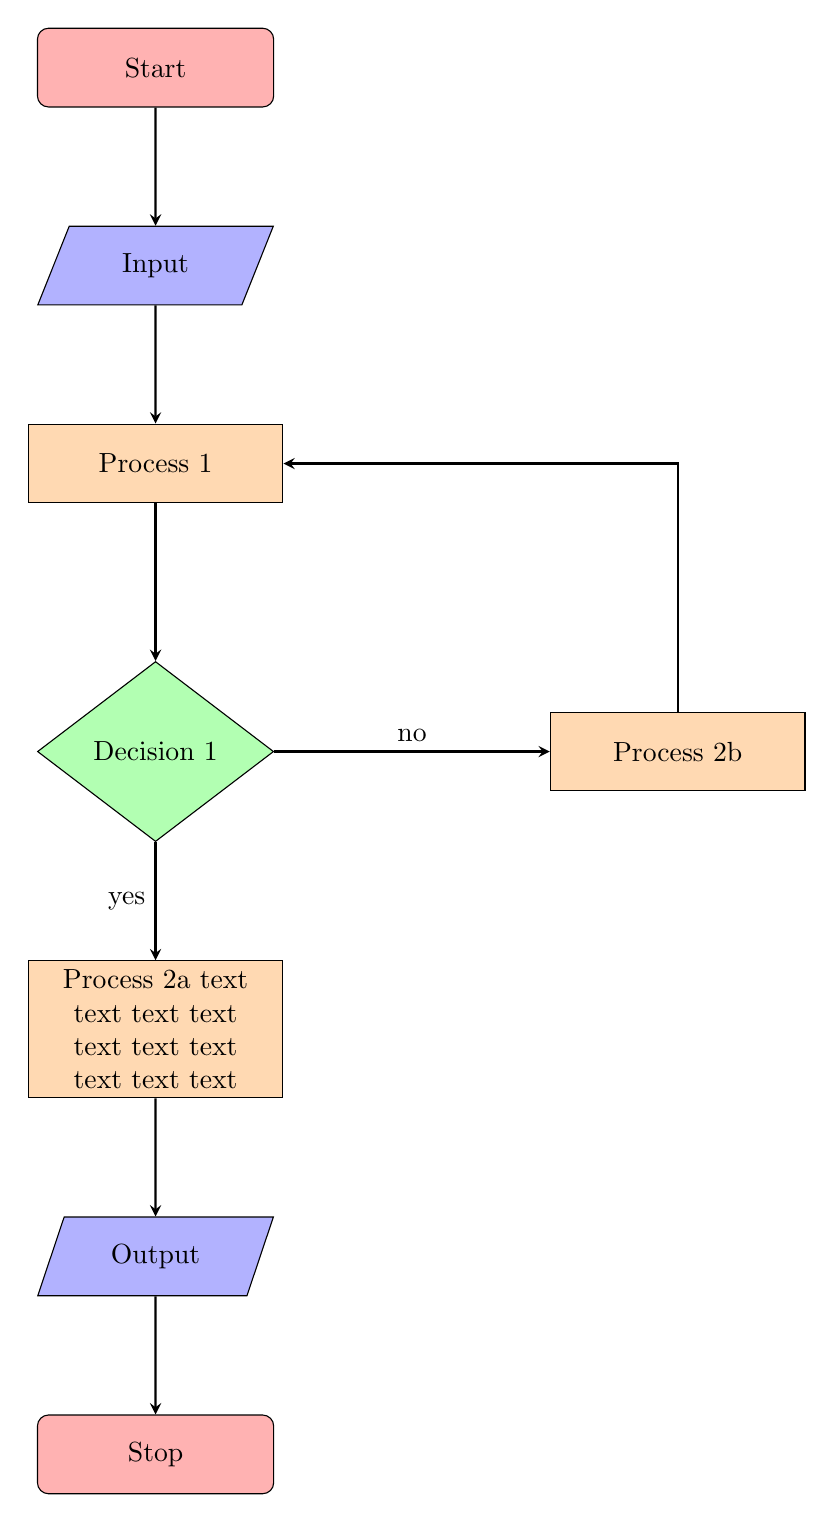
\begin{tikzpicture}[node distance=1.5cm]

\node [startstop] (start) {Start};
\node [io, below =of start] (in1) {Input};
\node [process, below= of in1] (pro1) {Process 1};
\node [decision, below=of pro1, yshift=-0.5cm] (dec1) {Decision 1};

\node [process, below= of dec1] (pro2a) {Process 2a
text text text text
text text text 
text text text};

\node (pro2b) [process, right = of dec1, xshift=2cm] {Process 2b};
\node (out1) [io, below = 1.5cm of pro2a] {Output};
\node (stop) [startstop, below = of out1] {Stop};

\draw [arrow] (start) -- (in1);
\draw [arrow] (in1) -- (pro1);
\draw [arrow] (pro1) -- (dec1);
\draw [arrow] (dec1) -- node[anchor=east] {yes} (pro2a);
\draw [arrow] (dec1) -- node[anchor=south] {no} (pro2b);
\draw [arrow] (pro2b) |- (pro1);
\draw [arrow] (pro2a) -- (out1);
\draw [arrow] (out1) -- (stop);

\end{tikzpicture}
\end{document}